\section{Resultados dos Modelos}

\subsection{Perceptron}

O perceptron é o modelo linear mais simples, pois apenas realiza uma combinação linear das \emph{features} e classifica o indivíduo de acordo com o sinal do resultado.
O melhor modelo encontrado utiliza regularização do tipo \emph{elastic-net}, com peso para regularização de Lasso igual a \( 0.3 \).
O peso para a regularização como um todo foi \( 0.001 \).

Na Figura \ref{perceptron metric} podemos ver a matriz de confusão e a curva ROC para este modelo.
As principais métricas do modelo foram:
\begin{itemize}
    \item \emph{Recall}: \( 90.7 \% \).
    \item Precisão: \( 32.8 \% \).
    \item Especificidade: \( 38.8 \% \).
    \item AUC: \( 0.648 \) (0.852 no treino).
\end{itemize}
\begin{figure}[htb]
    \begin{center}
        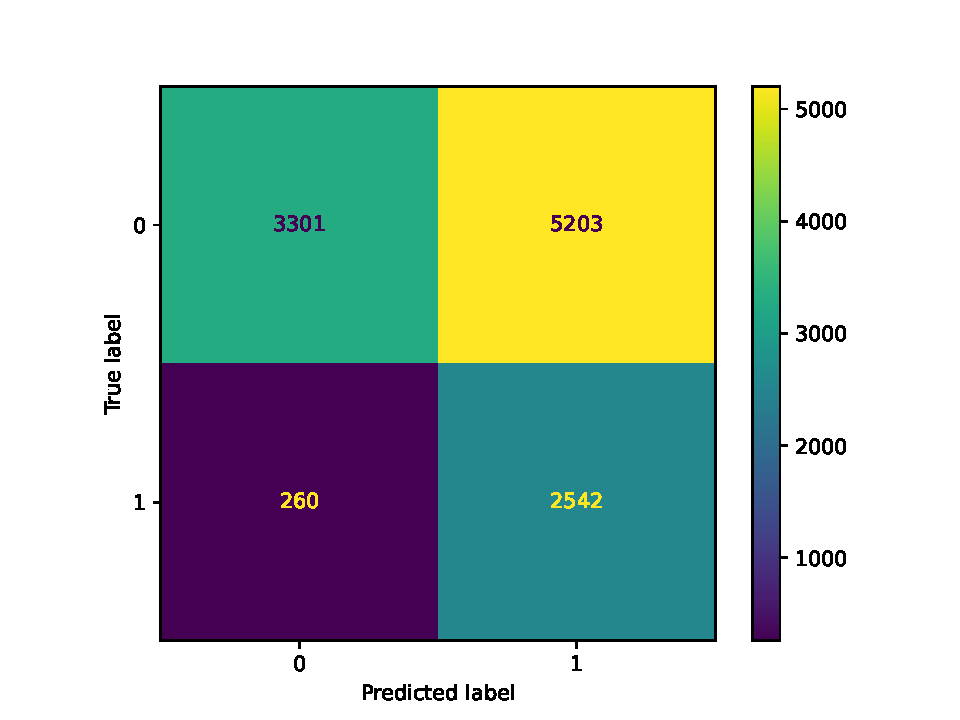
\includegraphics[width=.6\textwidth]{matrix_perceptron.pdf} \\
        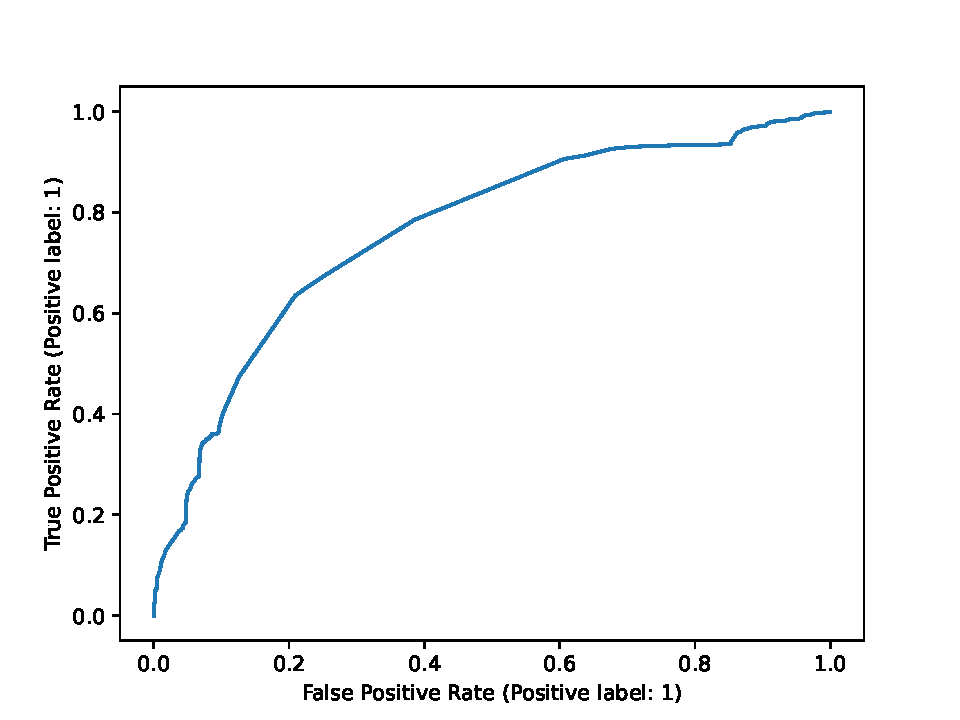
\includegraphics[width=.6\textwidth]{roc_curve_perceptron.pdf}
    \end{center}
    \caption{Matriz de confusão e curva ROC para o modelo perceptron. AUC = 0.648.}
    \label{perceptron metric}
\end{figure}

Para que os coeficientes tivessem valores significativos, o perceptron foi treinado com dados devidamente padronizados, para terem média zero e variância \( 1 \).
As \emph{features} com maiores pesos estão representadas na Figura \ref{perceptron feature}.
\begin{figure}[htb]
    \begin{center}
        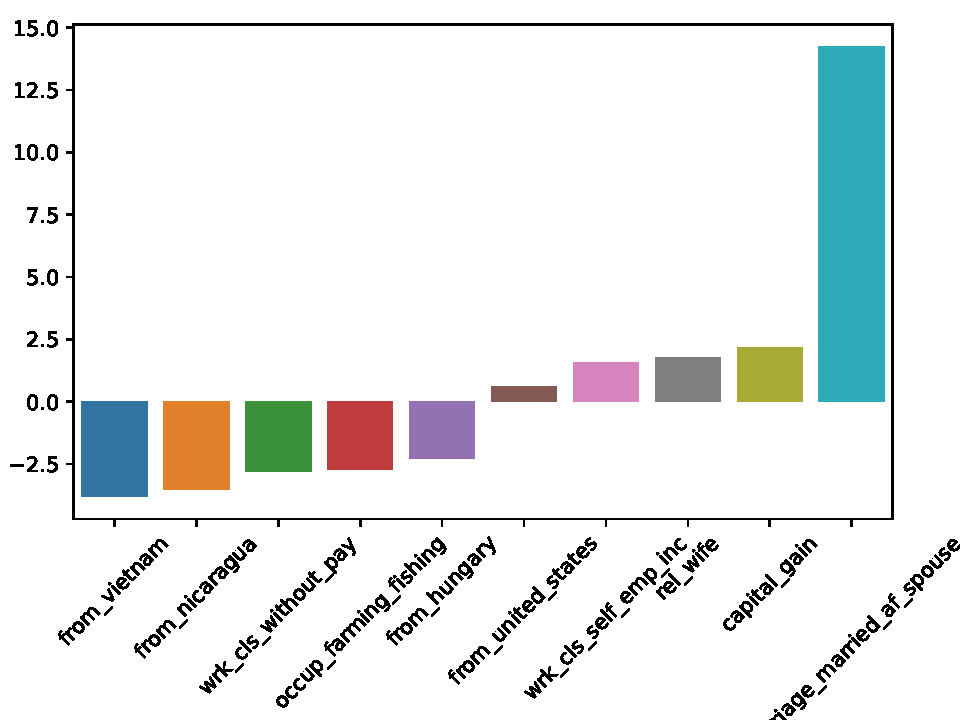
\includegraphics[width=.7\textwidth]{coefs_perceptron.pdf}
    \end{center}
    \caption{Feautures com maiores valores absolutos de pesos, positivos e negativos, para o perceptron.}
    \label{perceptron feature}
\end{figure}
Podemos ver claramente que, de acordo com o perceptron, ter um cônjuge nas forças aramadas (\verb|af| significa \emph{armed forces}) contribui de forma positiva para ter uma renda alta, enquanto ser do Vietnã, de forma negativa.
O campo \verb|capital_gain| não estava muito bem explicado na fonte do dataset, porém é razoável assumir que se trata dos ganhos monetários de fontes além do salário, como investimentos, por exemplo.

\subsection{Regressão Logística}

A Regressão Logística já é um modelo um pouco mais sofisticado, por usar uma ativação não linear.
Também utilizamos um \emph{Scaler} para padronizar os dados antes de cada chamada ao método \emph{fit}, de modo que os coeficientes possam ser utilizados para medir a relevância das \emph{features}.
O melhor modelo encontrado utiliza regularização do tipo \emph{elastic-net}, com peso para regularização de Lasso igual a \( 0.25 \).
A forma como o peso é dado para a regularazição como um todo é diferente do perceptron.
O termo da perda correspondente aos dados é multiplicado por uma constante \( C \), que, no caso do modelo validado, foi igual a \( 0.01 \), o que significa uma regularização bastante elevada.

Na Figura \ref{logit metric} podemos ver a matriz de confusão e a curva ROC para este modelo.
As principais métricas do modelo foram:
\begin{itemize}
    \item \emph{Recall}: \( 91.5 \% \).
    \item Precisão: \( 50.8 \% \).
    \item Especificidade: \( 70.7 \% \).
    \item AUC: \( 0.901 \) (0.904 no treino).
\end{itemize}
\begin{figure}[htb]
    \begin{center}
        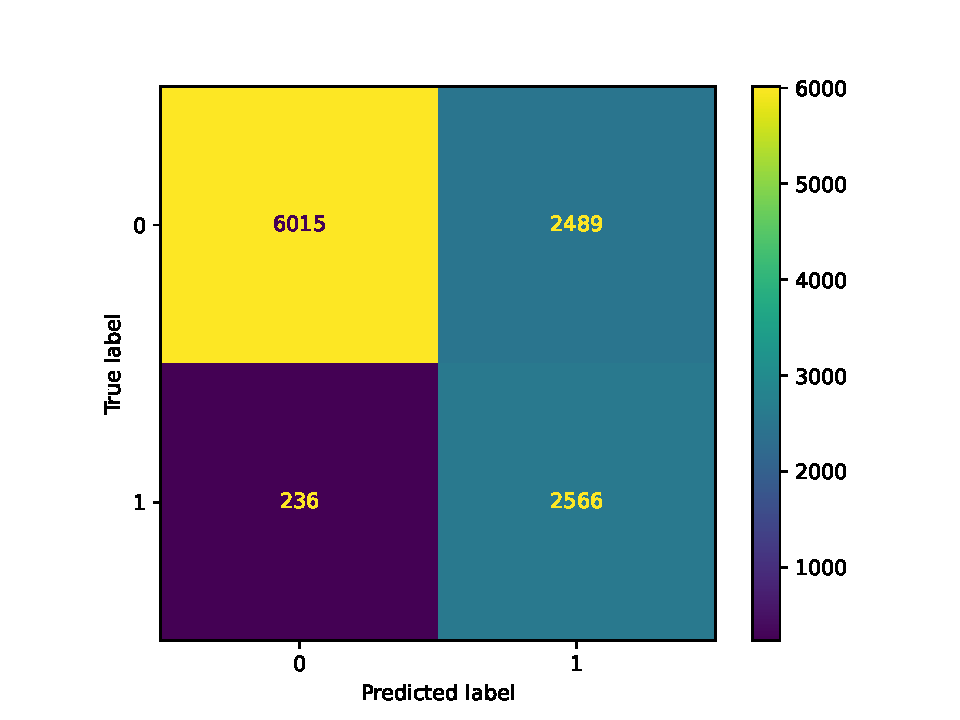
\includegraphics[width=.6\textwidth]{matrix_logit.pdf} \\
        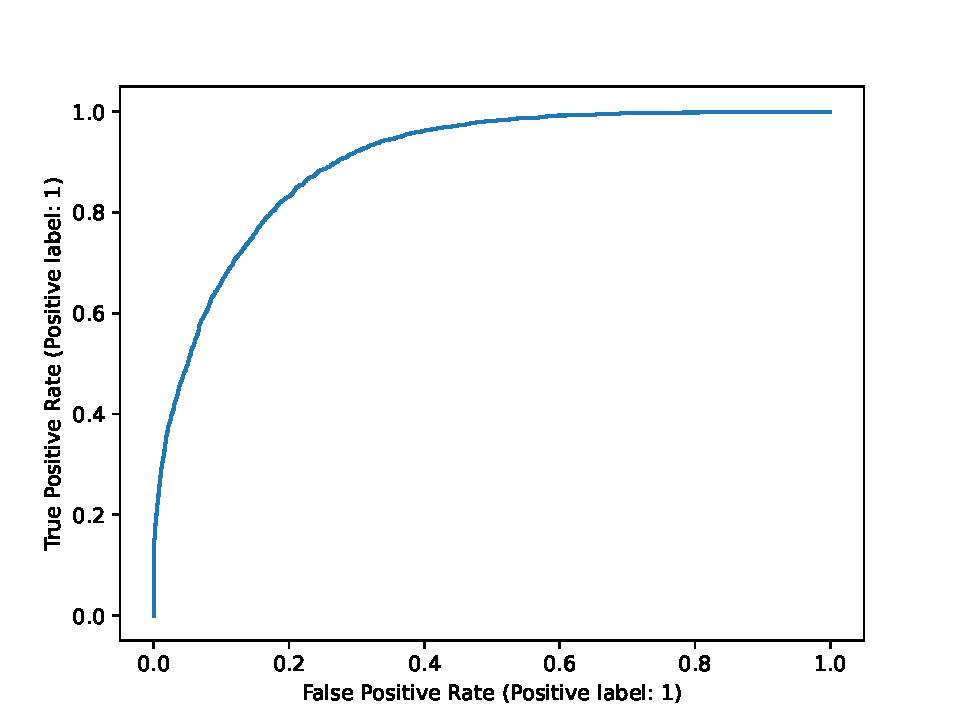
\includegraphics[width=.6\textwidth]{roc_curve_logit.pdf}
    \end{center}
    \caption{Matriz de confusão e curva ROC para o modelo de regressão logística. AUC = 0.901.}
    \label{logit metric}
\end{figure}
As \emph{features} com maiores pesos estão representadas na Figura \ref{logit feature}.
Por ela, concluímos que ter elevados ganhos de renda além do salário (\verb|capital_gain|), bem como ter uma boa educação, são fatores que contribuem para uma ter uma elevada renda.
Por outro lado, nunca ter se casado (\verb|marriage_never_married|) contribui negativamente.
\begin{figure}[htb]
    \begin{center}
        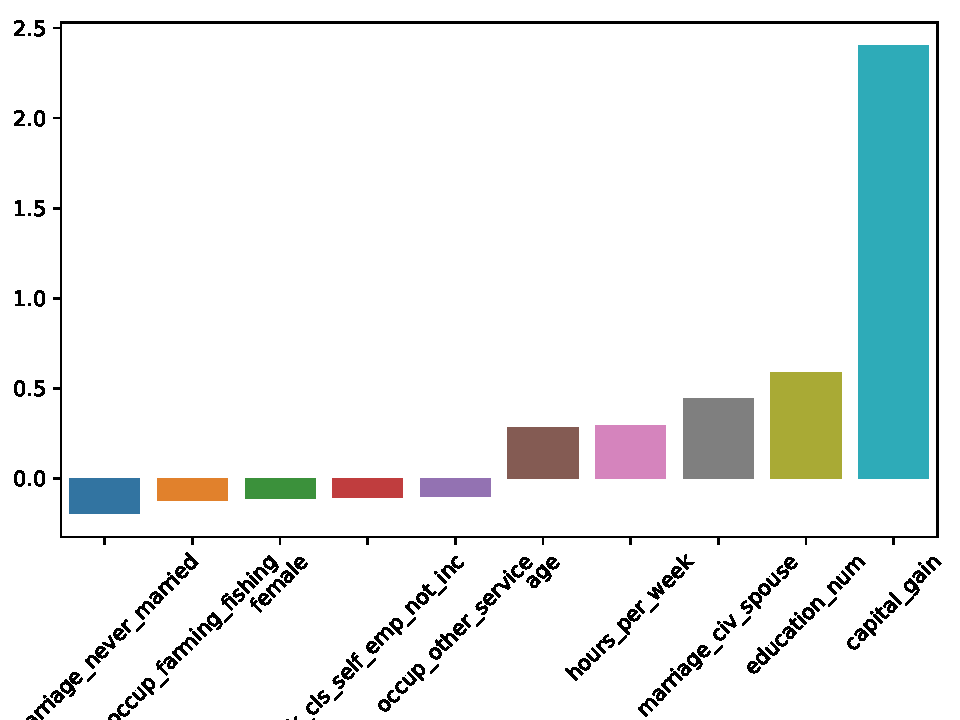
\includegraphics[width=.7\textwidth]{coefs_logit.pdf}
    \end{center}
    \caption{Feautures com maiores valores absolutos de pesos pesos, positivos e negativos, para a regressão logística.}
    \label{logit feature}
\end{figure}

\subsection{Modelos baseados em árvores}

Para os modelos baseados em árvores, uma desvantagem comparativa foi o fato de que a implementação de árvores do \emph{Sci-Kit Learn} não suporta \emph{features} binárias, como é possível ver no último parágrafo \href{https://scikit-learn.org/stable/modules/tree.html#tree-algorithms-id3-c4-5-c5-0-and-cart}{desta seção (1.10.6)} do \emph{user guide} do \emph{Sci-Kit Learn}.
Para confirmar isso, ao tentarmos treinar com variáveis categóricas, geramos uma falha, pois o algoritmo esparava apenas floats.

\subsubsection{Uma árvore}

Com o intuito de começar simples e depois complicar, primeiro treinamos uma única árvore.
Os melhores parâmetros escolhidos por validação cruzada foram:
\begin{itemize}
    \item Um \( \alpha \) relativo à poda de custo-complexidade igual a \( 0.001 \).
    \item  Profundidade máxima igual a \( 9 \).
    \item Um mínimo de \( 1 \% \) de samples em cada folha.
\end{itemize}

Na Figura \ref{single tree metric} podemos ver a matriz de confusão e a curva ROC para este modelo.
As principais métricas do modelo foram:
\begin{itemize}
    \item \emph{Recall}: \( 49.9 \% \).
    \item Precisão: \( 70.2 \% \).
    \item Especificidade: \( 93.0 \% \).
    \item AUC: \( 0.84 \) (0.844 no treino).
\end{itemize}
\begin{figure}[htb]
    \begin{center}
        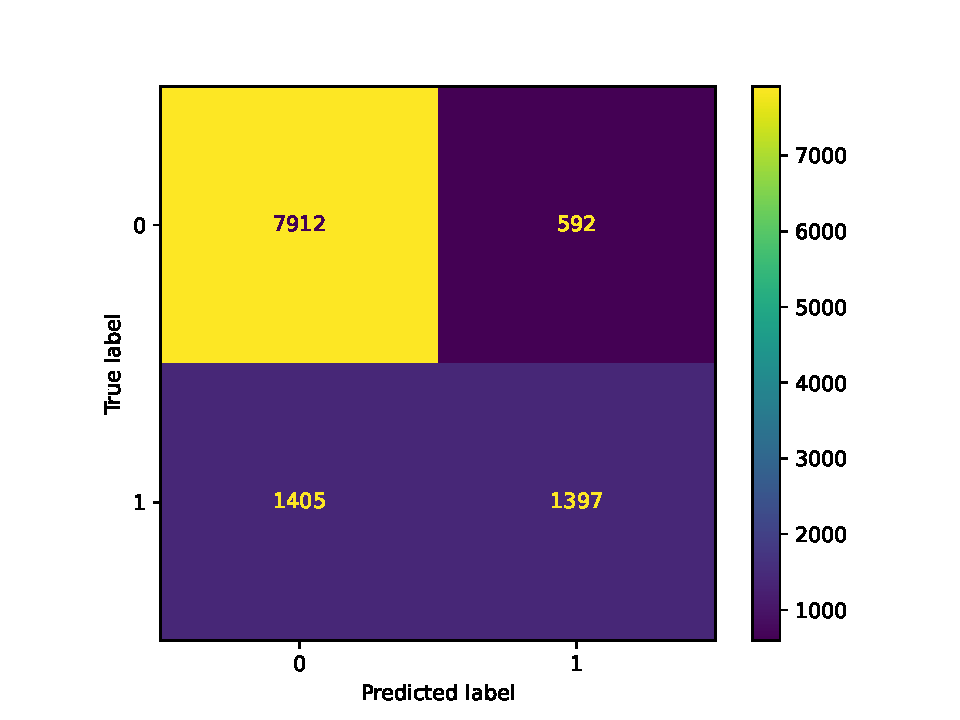
\includegraphics[width=.6\textwidth]{matrix_single_tree.pdf} \\
        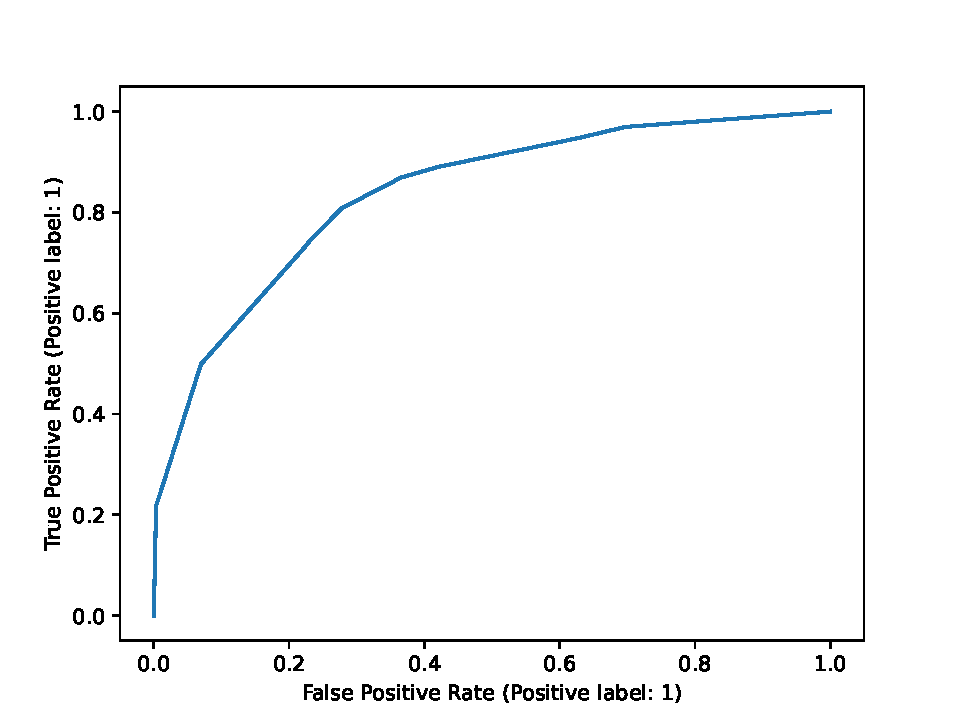
\includegraphics[width=.6\textwidth]{roc_curve_single_tree.pdf}
    \end{center}
    \caption{Matriz de confusão e curva ROC para uma única árvore. AUC = 0.838.}
    \label{single tree metric}
\end{figure}

As \emph{features} com mais importância estão retratadas na Figura \ref{single tree feature}.
Essa importância é calculada como sendo a redução total da perda, normalizada, causada por aquela \emph{feature}.
Podemos ver que, de acordo com uma única árvore, o grau de educação de um indivíduo e a sua idade são duas boas variáveis para explicar a sua renda.
\begin{figure}[htb]
    \begin{center}
        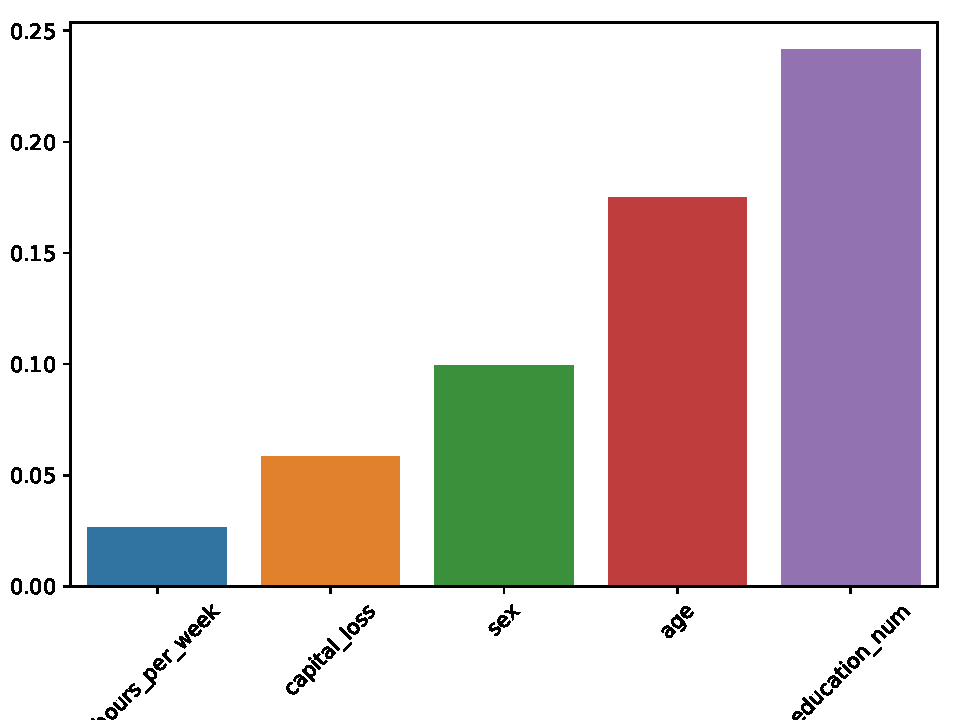
\includegraphics[width=.7\textwidth]{single_tree_feature_importances.pdf}
    \end{center}
    \caption{Features com maiores importâncias, de acordo com uma única árvore.}
    \label{single tree feature}
\end{figure}
Por se tratar de apenas \emph{uma} árvore, podemos representá-la graficamente, o que é feito na Figura \ref{plot tree}
\begin{figure}[htb]
    \begin{center}
        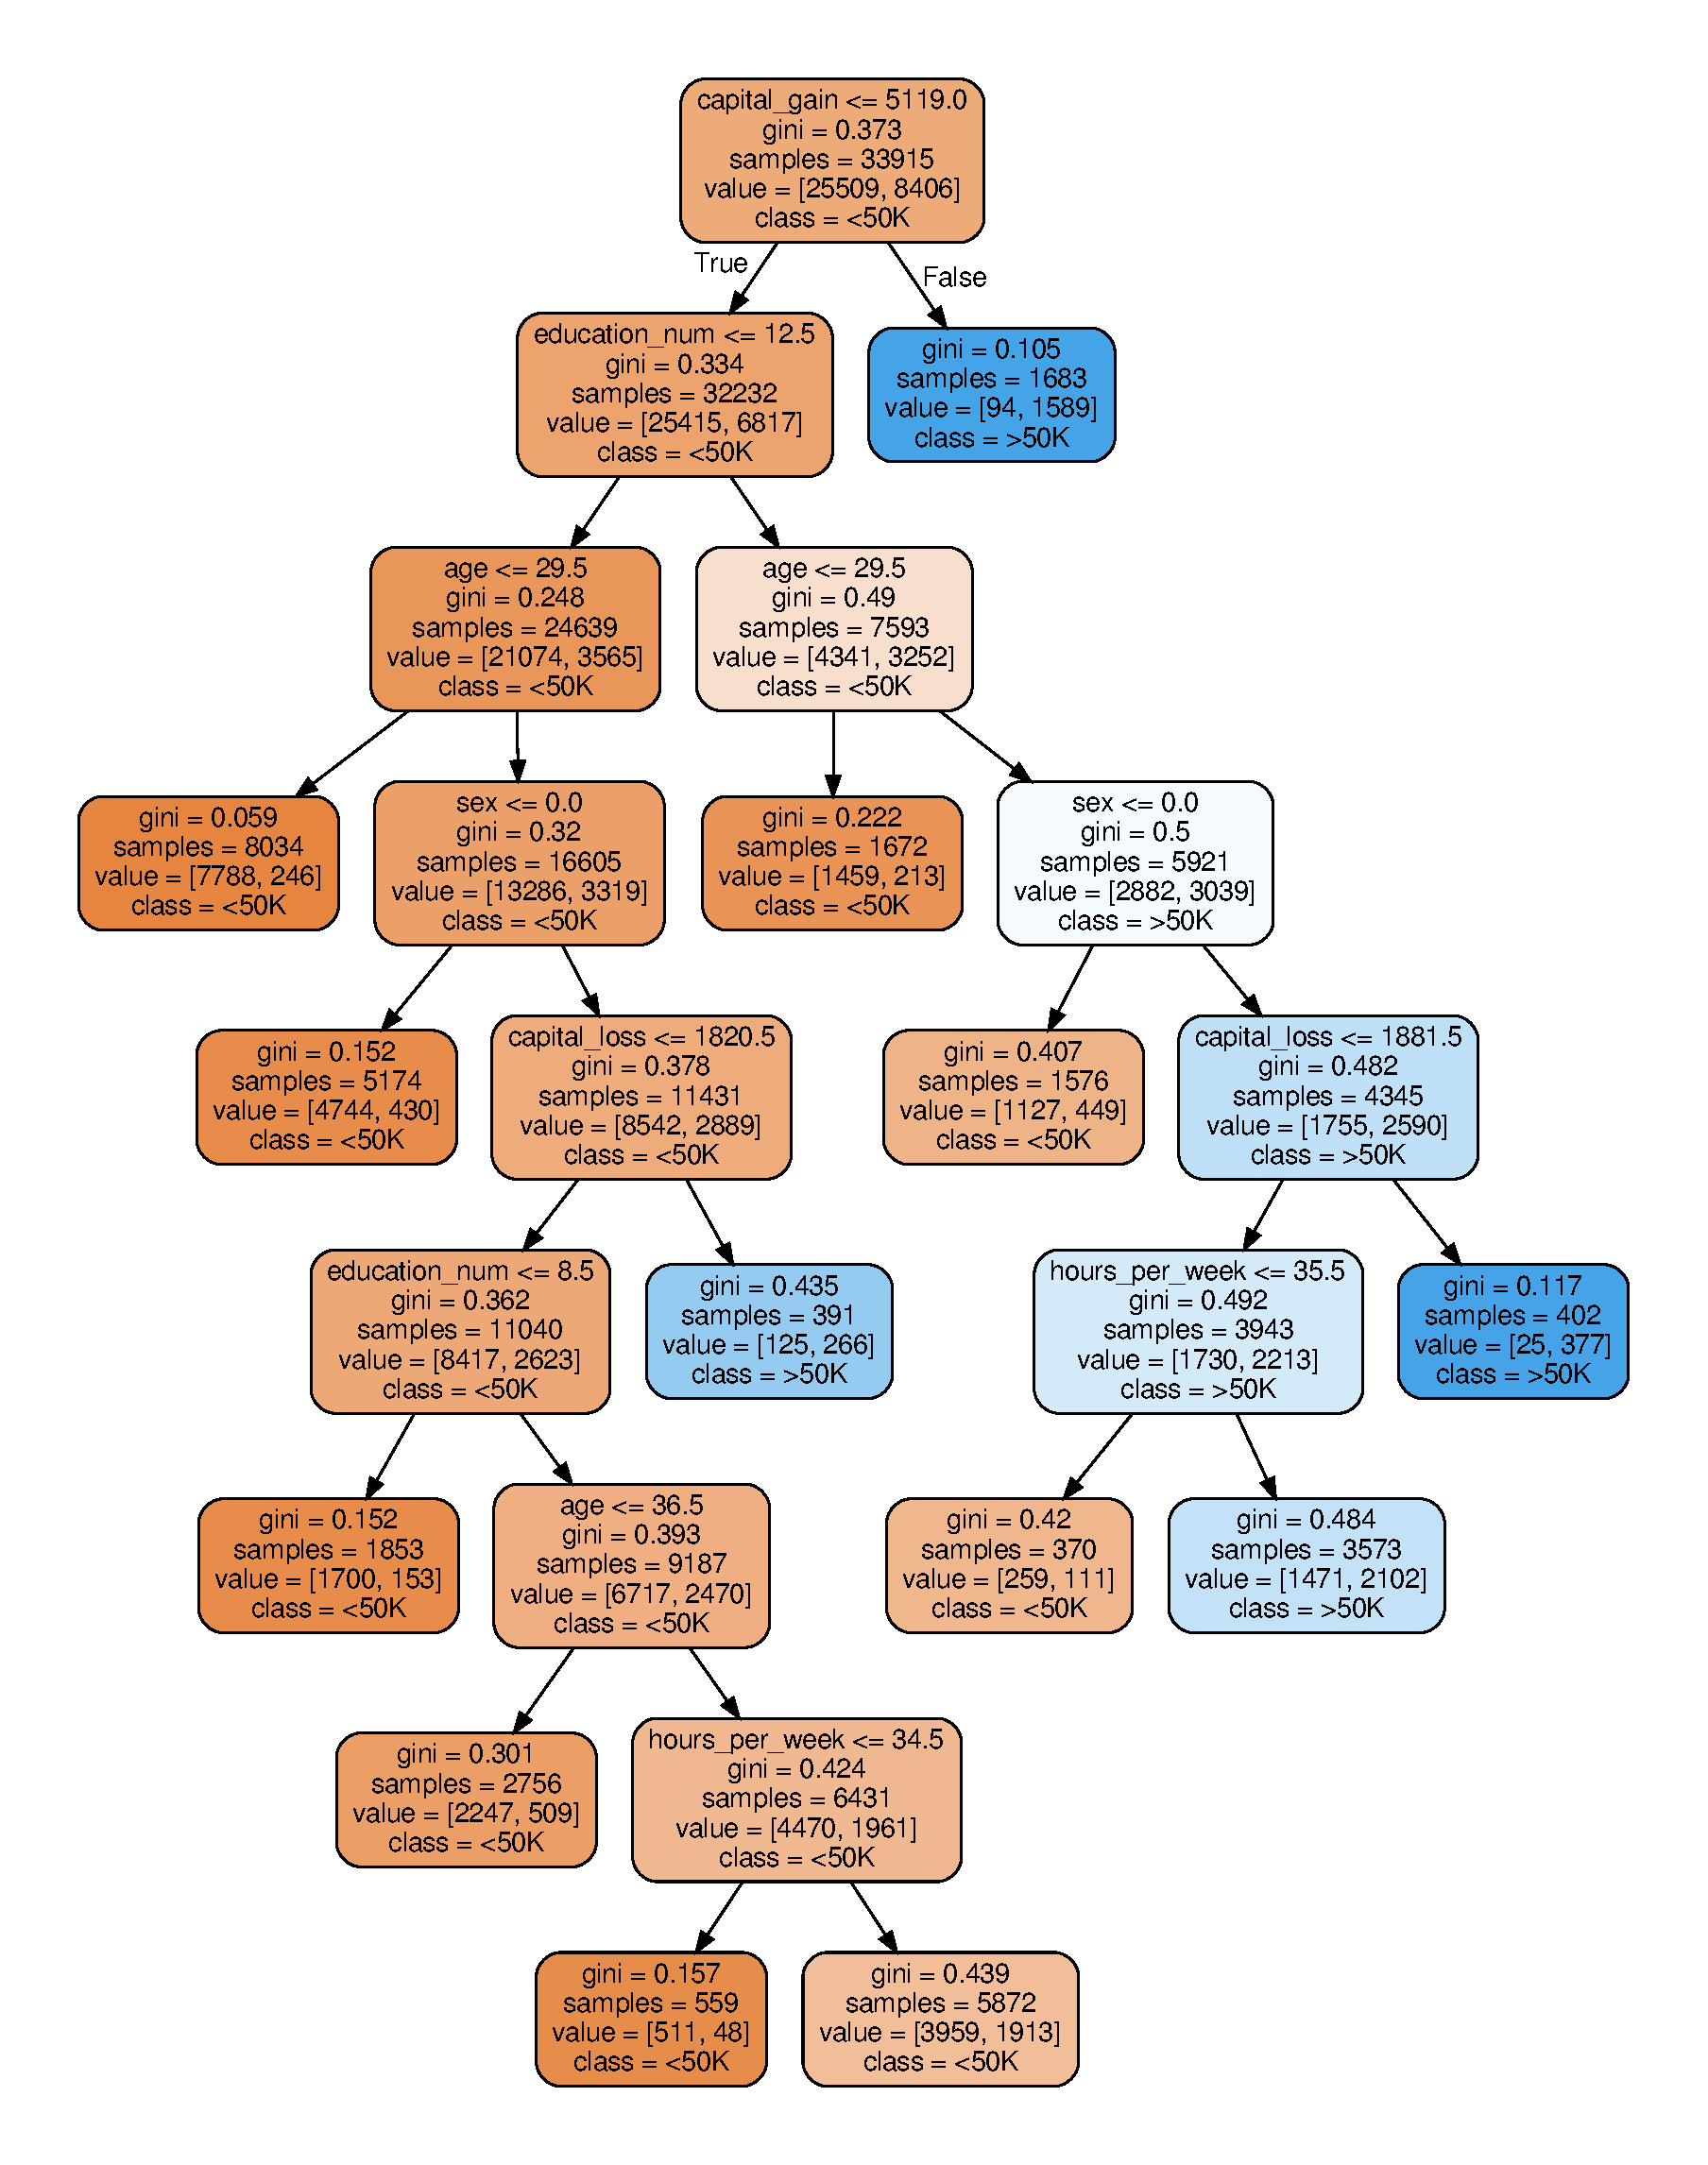
\includegraphics[width=\textwidth]{tree/Source.gv.pdf}
    \end{center}
    \caption{Árvore obtidas ao fitarmos apenas um classificador no dataset.}
    \label{plot tree}
\end{figure}

\subsubsection{\emph{Bag of trees}}

O próximo passo é o de ajustar um \emph{bagging} classifier nos dados, utilizando árvores como classificadores básicos.
Esse tipo de estimdor tem como objetivo reduzir a variância do modelo, de modo que se espera que ele generalize melhor.
Por uma questão de falta de recursos computacionais, como parâmetros para cada classificador dentro do \emph{bag}, utilizamos os melhores parâmetros encontrados por validação cruzada para uma única árvore.
Com relação ao número de estimadores, vemos que, como esperado, quanto mais estimadores utilizamos, melhor é o desempenho do modelo.
Entretanto, a partir de cerca de \( 100 \) estimadores, o ganho marginal começou a ser muito pequeno.

Na Figura \ref{bag of trees metric} podemos ver a matriz de confusão e a curva ROC para este modelo.
As principais métricas do modelo foram:
\begin{itemize}
    \item \emph{Recall}: \( 27.4 \% \).
    \item Precisão: \( 89.1 \% \).
    \item Especificidade: \( 99 \% \).
    \item AUC: \( 0.856 \) (0.862 no treino).
\end{itemize}
\begin{figure}[htb]
    \begin{center}
        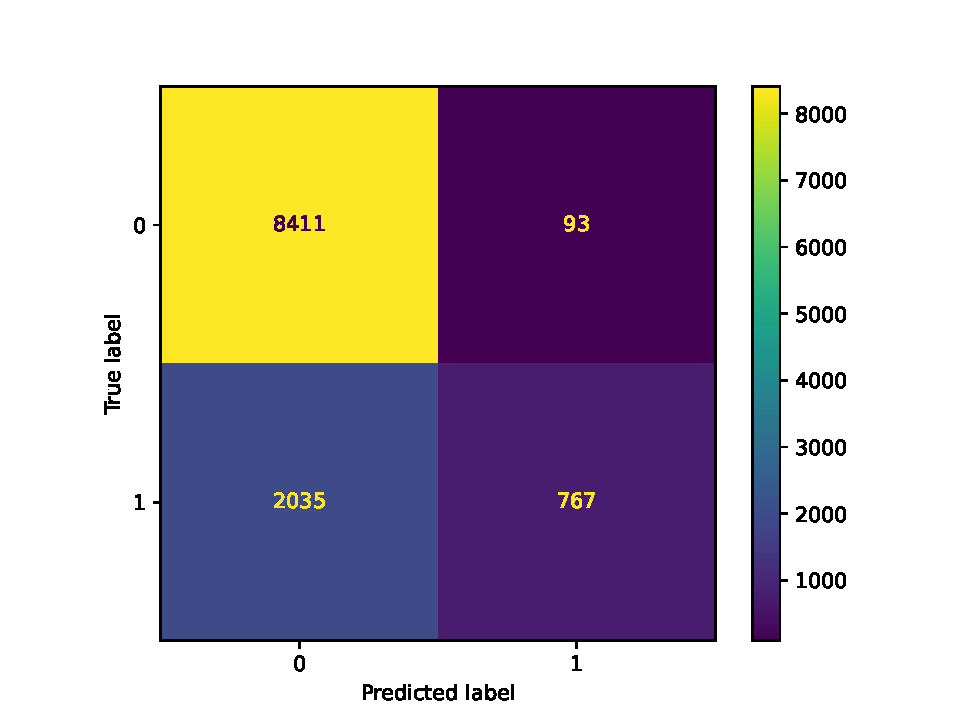
\includegraphics[width=.6\textwidth]{matrix_bag_of_trees.pdf} \\
        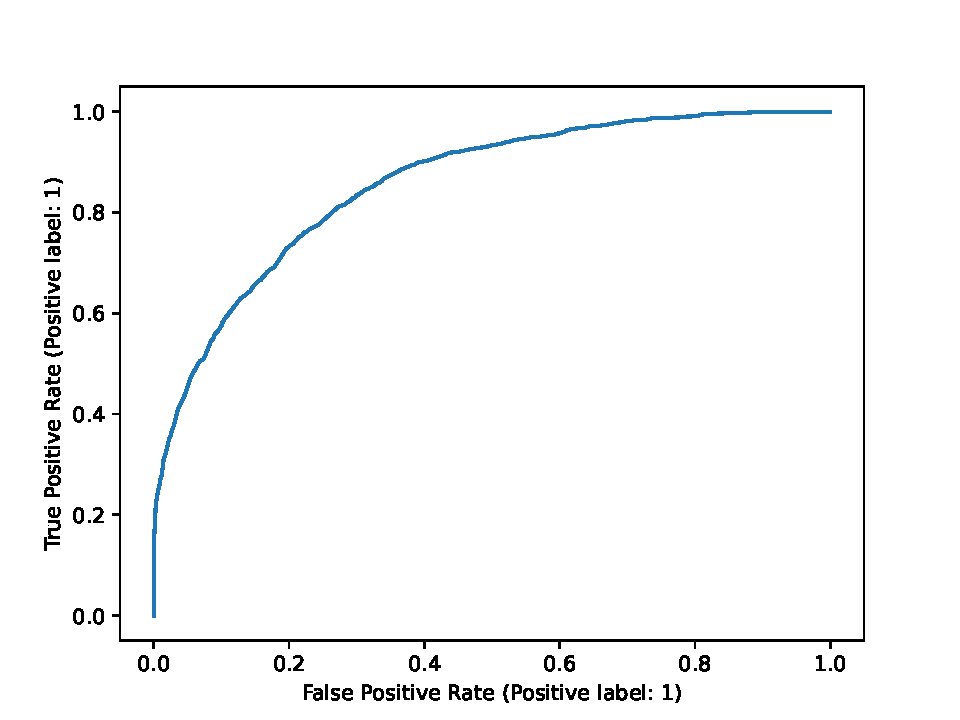
\includegraphics[width=.6\textwidth]{roc_curve_bag_of_trees.pdf}
    \end{center}
    \caption{Matriz de confusão e curva ROC para um \emph{bag of trees}. AUC = 0.856.}
    \label{bag of trees metric}
\end{figure}
Vemos que, apesar do \emph{recall} ter caído, todas as outras métricas subiram.

\subsubsection{\emph{Random Forest}}

O \emph{random forest} é um \emph{bag}, porém com uma tentativa de descorrelacionar as árvores.
Todas as considerações feitas para o \emph{bag of trees} se aplicam aqui.

Na Figura \ref{random forest metric} podemos ver a matriz de confusão e a curva ROC para este modelo.
As principais métricas do modelo foram:
\begin{itemize}
    \item \emph{Recall}: \( 46.9 \% \).
    \item Precisão: \( 72.27 \% \).
    \item Especificidade: \( 94.06 \% \).
    \item AUC: \( 0.855 \) (0.859 no treino).
\end{itemize}
\begin{figure}[htb]
    \begin{center}
        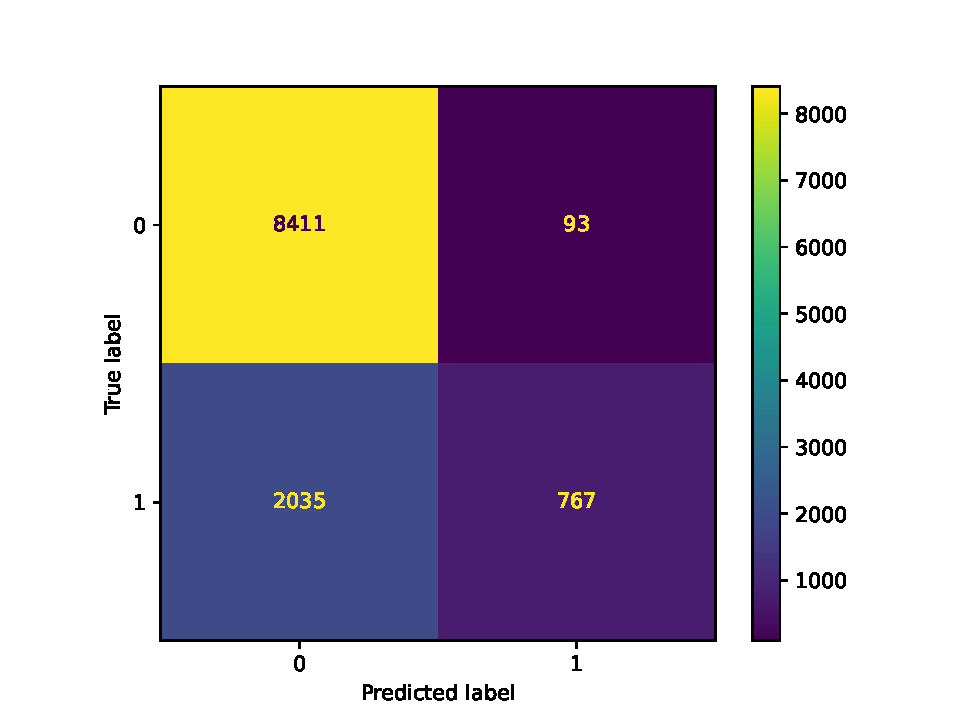
\includegraphics[width=.6\textwidth]{matrix_bag_of_trees.pdf} \\
        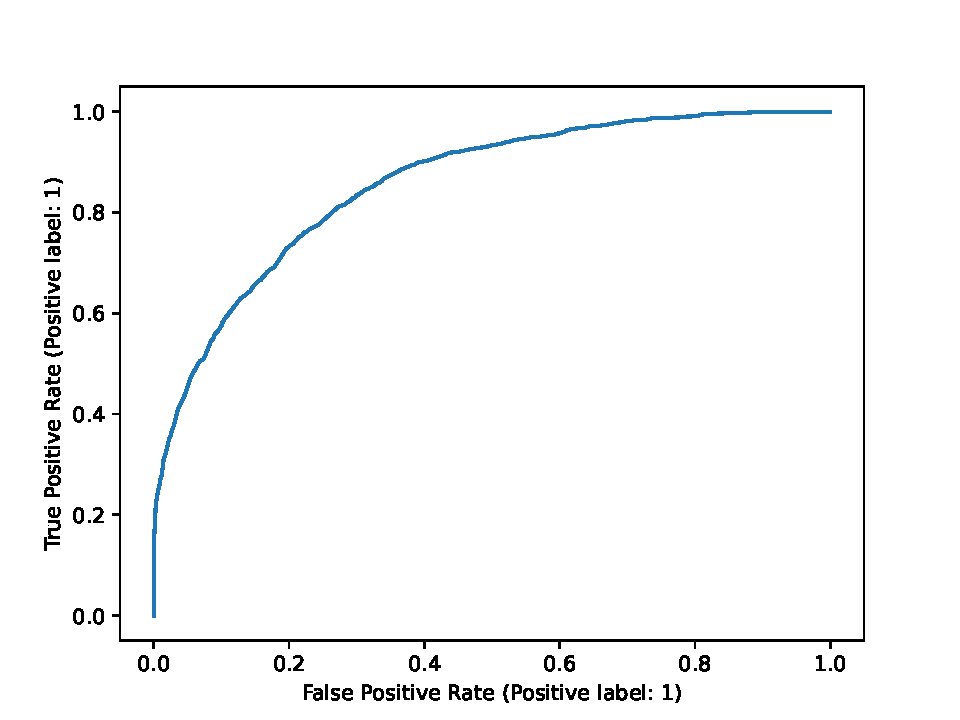
\includegraphics[width=.6\textwidth]{roc_curve_bag_of_trees.pdf}
    \end{center}
    \caption{Matriz de confusão e curva ROC para um \emph{bag of trees}. AUC = 0.856.}
    \label{random forest metric}
\end{figure}
Podemos ver que, apesar de uma queda na precisão e na especificidade com relação ao modelo de \emph{bagging}, houve um aumento do \emph{recall}, de modo que podemos concluir que o modelo ficou mais balanceado.

Para o \emph{random forest}, novamente temos uma forma prática de calcular as importâncias de cada \emph{feature}, já disponível como um método no \emph{Sci-Kit Learn}.
Ela é exatamente a mesma do classificador com apenas uma árvore.
As \emph{features} mais importamentes de acordo com essa métrica estão representadas na Figura \ref{random forest feature}.
\begin{figure}[htb]
    \begin{center}
        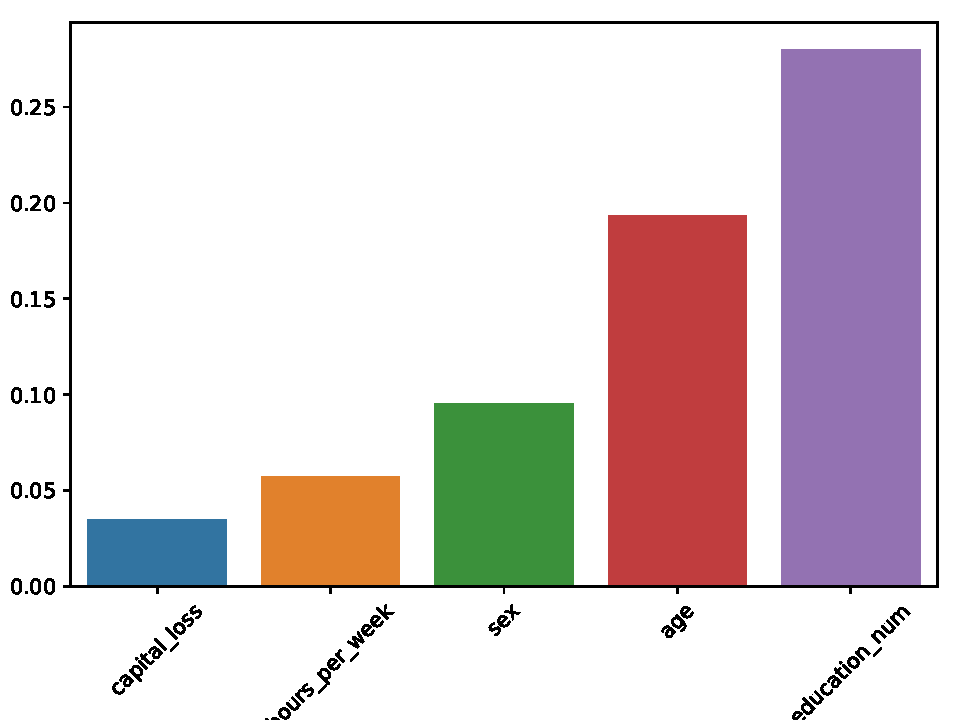
\includegraphics[width=.7\textwidth]{random_forest_feature_importances.pdf}
    \end{center}
    \caption{Features com maiores importâncias, de acordo com uma \emph{random forest}.}
    \label{random forest feature}
\end{figure}
Vemos que as conclusões são exatamente as mesmas obtidas quando consideramos apenas uma árvore.

\subsection{SVM}

As \emph{Support Vector Machines} são a classe de modelos mais complexa que consideramos.
Utilizamos um SVC (\emph{Support Vector classifier}) em conjunção com um \emph{scaler}.
Fizemos um \emph{grid search} para encontrar o melhor \emph{kernel} e parâmetro de regularização.
O resultado obtido foi um \emph{kernel} linear, com parâmetro de regularização \( C = 1 \) (veja a seção sobre regressão logística).
Como o \( SVM \) não gera probabilidades, a validação cruzada não foi realizada com a métrica AUC, e sim com a \emph{balanced accuracy score}, que, como dito na seção anterior, é a média entre o \emph{recall} e a especificidade.
As principais métricas do modelo foram:
\begin{itemize}
    \item \emph{Recall}: \( 85.55 \% \).
    \item Precisão: \( 57.70 \% \).
    \item Especificidade: \( 77.59 \% \).
    \item \emph{balanced accuracy score}: \( 0.816 \) (0.813 no treino).
\end{itemize}
Podemos ver que o modelo se saiu melhor no teste do que no treino.
Também vemos que ele apresenta um conjunto de métricas muito bom, comparado aos outros classificadores, por ser o único que conseguiu tanto \emph{recall} quanto especificidade elevados.
Na Figura \ref{svm metric} podemos ver a matriz de confusão para este modelo.
\begin{figure}[htb]
    \begin{center}
        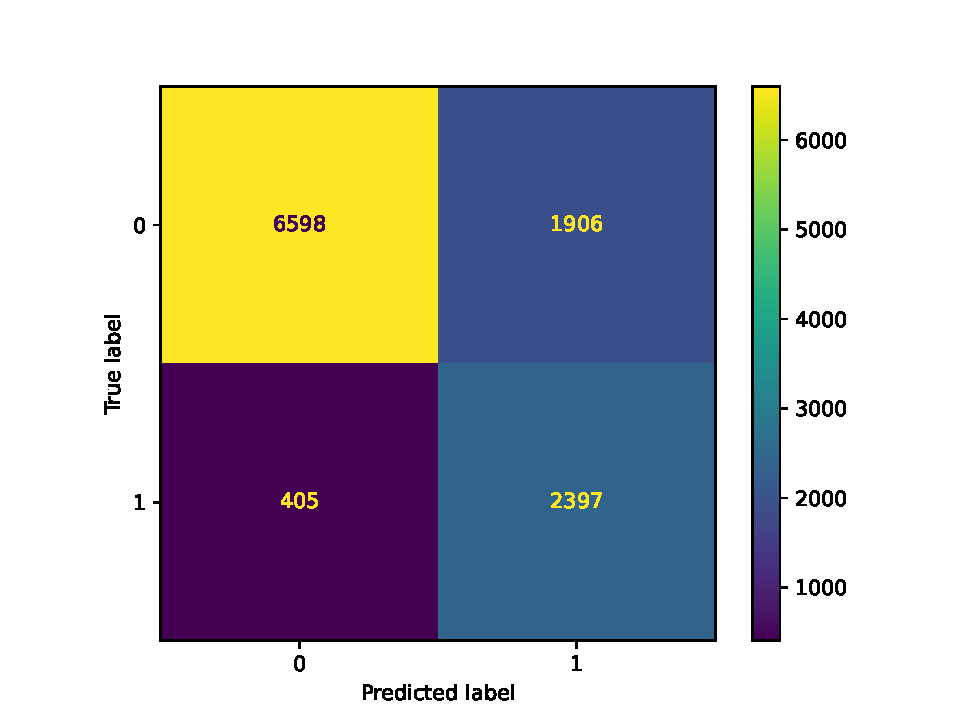
\includegraphics[width=.6\textwidth]{matrix_svm.pdf} \\
    \end{center}
    \caption{Matriz de confusão para o SVM.}
    \label{svm metric}
\end{figure}
